\chapter{\IfLanguageName{dutch}{Stand van zaken}{State of the art}}%
\label{ch:stand-van-zaken}

% Tip: Begin elk hoofdstuk met een paragraaf inleiding die beschrijft hoe
% dit hoofdstuk past binnen het geheel van de bachelorproef. Geef in het
% bijzonder aan wat de link is met het vorige en volgende hoofdstuk.

% Pas na deze inleidende paragraaf komt de eerste sectiehoofding.


\section{Data Leakage Prevention (DLP)}%

Een DLP-systeem heeft als doel drie soorten gegevens binnen een organisatie te beschermen: data-at-rest, data-in-motion en data-in-use. 
Data-at-rest verwijst naar statische informatie die is opgeslagen in bedrijfssystemen, zoals documentbeheersystemen, e-mailservers, bestandsservers, netwerkschijven, 
persoonlijke computers en opslagruimtenetwerken (SANs). 
Data-in-motion verwijst naar bedrijfsdata dat wordt verwerkt binnen het uitgaande netwerkverkeer, zoals e-mails en online verkeer. 
Data-in-use bestaat uit informatie die medewerkers gebruiken op eindgebruikersapparaten, zoals een bestand kopiëren naar een USB-schijf. 
De definitie van vertrouwelijkheid binnen een organisatie vereist een grondigere analyse. 
Soorten informatie zoals PII, inclusief namen, identiteitskaart- en creditcardgegevens, worden doorgaans in elke organisatie als vertrouwelijk beschouwd.
Deze definitie krijgt echter ingewikkeldere aspecten bij bedrijfsgeheimen en interne communicatie, die vaak onregelmatig zijn. 
Vertrouwelijke informatie verwijst naar gegevens die binnen de organisatie zijn verzameld en niet algemeen toegankelijk zijn. 
Een DLP-systeem bevat de mogelijkheid om gevoelige gegevens te herkennen in een of meerdere van de genoemde datatypen.

\subsection{PCI en PII}

Persoonlijk identificeerbare informatie (PII), zoals namen, rijksregisternummers, e-mail\-adressen, telefoonnummers en dergelijke kunnen direct of indirect worden gebruikt voor de identificatie van een persoon. 
Met het oog op de AVG zijn er strikte regels met betrekking tot toestemming en transparantie bij de verwerking van PII. 
Payment Card Industry (PCI)-gegevens bevatten alle kaart- en betaalgegevens zoals debit-/creditcardnummers, Primary Account Numbers (PAN) en andere confidentiële authenticatiegegevens zoals CVV. 
Om te voldoen aan de PCI DSS-norm (Payment Card Industry Data Security Standard), 
moeten organisaties strenge maatregelen implementeren om deze kaartgegevens te beveiligen. 
Bedrijven die persoonlijk identificeerbare informatie (PII) en PCI-data verwerken lopen het risico op zware sancties als deze gegevens niet voldoende beschermd worden.

\subsection{Detectie methoden voor gegevensverlies}

Identificatiemiddelen worden gebruikt om gevoelige informatie, zoals PII en PCI, te detecteren. 
Dit gebeurt op basis van reguliere expressies (regex). 
Regex is een krachtig hulpmiddel dat DLP helpt specifieke gegevenstypen te herkennen door middel van uitdrukkingen, termen en patronen, 
zoals \texttt{BE\textbackslash d\{2\}\textbackslash s?\textbackslash d\{4\}\textbackslash s?\textbackslash d\{4\}\-\textbackslash s?\textbackslash d\{4\}} 
dat kan dienen voor Belgische IBAN-codes. 
Hoewel dit patroon effectief is voor standaard IBAN-formaten, 
kan het worden omzeild door een karakter toe te voegen in de invoer, wat het belang benadrukt van extra controles. 

De aangemaakte identificatie voor confidentiële gegevens moet voldoen aan de volgende richtlijnen:

\begin{itemize}
    \item Vooraf gedefinieerde en aanpasbare patronen voor datadetectie: Het is cruciaal om duizenden vooraf ingestelde regels voor het herkennen van gegevens beschikbaar te hebben en deze te kunnen aanpassen aan de behoeften van de organisatie.
    \item Ondersteuning voor verschillende soorten bestandstypen (Word, Excel, PDF, JPG, PNG, CSV, ZIP en RAR, enz.) en categorieën (afbeeldingen, databases, spreadsheets, enz.).
    \item Ondersteuning voor landspecifieke identificatienummers (IBAN's, postcodes, adressen, nationale identiteitskaarten, IP-adressen, pas\-poort- en telefoonnummers).
    \item Voldoen aan de wet- en regelgeving.
\end{itemize}

De bescherming van PII en PCI-gegevens vormt een kernaspect van DLP. \textcite{Wason2020CASB} legt de nadruk op het belang van de integratie van Cloud Access Security Brokers (CASB) in cloudomgevingen. 
CASB biedt organisaties de mogelijkheid om een uitgebreide zichtbaarheid te krijgen in het gebruik van cloudtoepassingen, inclusief goedgekeurde en ongeautoriseerde (shadow IT) diensten. 
Het houdt bij hoe de confidentiële data wordt opgeslagen en verplaatst/verwerkt, wat handig is voor het identificeren van deze data en het voorkomen van datalekken.

\subsection{\IfLanguageName{dutch}{Regelsets}{Rule sets}}
\label{subsec:regelsets-literatuurstudie}

De regelsets binnen Netskope zijn de focus van dit onderzoek. Deze bestaan uit een combinatie van verschillende identificatiemethoden, zoals beschreven in de documentatie van \textcite{Netskope2025DLP}. 
Deze identificatoren of ook entiteiten genoemd, zijn de basis van DLP-regels en vormen samen een regelset. 
Meerdere regelsets kunnen worden gedefinieerd binnen een profiel \autocite{Netskope2025Profiles}.


% A DLP profile is a collection of predefined or custom DLP rules, classifiers, and custom fingerprint rules. If any of the rules or classifiers match the content, then the DLP profile flags the content as a policy violation. Using predefined profiles let you start evaluating loss of critical data in the cloud immediately. Creating new DLP profiles and rules enables you to refine custom methods of prevention. For insight about building custom DLP profiles and rules, see DLP Best Practices Runbook.

\textbf{Tabel naar Nederlands}

{\small
\begin{itemize}
    \item \textbf{Predefined data identifiers}: Dit zijn vooraf gedefinieerde identificatoren die zijn ontworpen door Netskope.
    \item \textbf{Custom data identifiers}: Dit zijn op maat gemaakte identificatoren die organisaties kunnen definiëren om specifieke soorten gevoelige gegevens te herkennen die relevant zijn voor hun bedrijfsvoering.
    \item \textbf{Keyword identifiers}: Dit zijn specifieke woorden of zinnen die worden gebruikt om gevoelige gegevens te identificeren. Dit kan bijvoorbeeld een lijst zijn van veelvoorkomende achternamen die in combinatie met een rijksregisternummer kunnen worden gebruikt.
    \item \textbf{Regular expressions (RegEx)}: Dit zijn patronen die worden gebruikt om specifieke gegevensformaten te identificeren. RegEx kan worden gebruikt om complexe gegevensstructuren te herkennen, zoals IBAN-nummers of e-mailadressen.
    \item \textbf{Exact match criteria}: Dit zijn specifieke voorwaarden die moeten worden vervuld om te bepalen of een gegevenstype als gevoelig wordt beschouwd, zoals 
\end{itemize}
}


\subsubsection{\IfLanguageName{dutch}{Vooraf gedefinieerde regelsets}{Predefined rules}}
\label{subsubsec:vooraf-gedefinieerde-regels-literatuurstudie}

Netskope biedt een uitgebreide set vooraf gedefinieerde regelsets binnen zijn DLP-functionaliteit. 
Hiermee kan gevoelige informatie, zoals PII en PCI, effectief worden gedetecteerd en beschermd.
Volgens \textcite{brouwer2021cloud} heeft Netskope een uitgebreide lijst van DLP-profielen ontwikkeld die helpen bij het identificeren van allerlei soorten PII,
verschillend van EU-identificatiegegevens tot Singaporese identificatiegegevens en medische rapporten. 
Deze regelsets zijn uitgebalanceerd en sluiten aan bij de regelgeving van de meeste westerse landen. 

Deze vooraf gedefinieerde regelsets zijn niet veranderbaar en kunnen niet verder worden gepersonaliseerd. 
Gebruikers kunnen echter wel hun eigen DLP-profielen definiëren voor specifieke use-cases, zoals in volgende sectie wordt besproken. 

Een voorbeeld van een vooraf gedefinieerde regelset is de regelset voor 'DLP-PII', die is ontworpen om gevoelige persoonlijke informatie te identificeren en te beschermen. 
Deze regelset omvat gegevens zoals naam, adres, geboortedatum, e-mailadres, MedicareID, paspoortinformatie en sociale zekerheidsnummers. Alleen zijn deze specifiek gericht voor de Verenigde Staten en Canada. 
Aangezien dit onderzoek zich richt op de bescherming van Belgische persoons\-- en betalingsgegevens, voldoet deze regelset niet aan de vereisten van de Belgische wetgeving.

Daarnaast biedt Netskope ook de 'EU General Data Protection Regulation (GDPR)' regelset aan, die specifiek is ontworpen om te voldoen aan al de vereisten van de AVG. 
Deze regelset richt zich op persoonsgegevens van een natuurlijk persoon binnen de Europese Unie. 
In Tabel \ref{tab:EU-AVG Netskope} zijn de gegevenscategorieën weergegeven die Netskope heeft gedefinieerd voor deze regelset \autocite{Netskope2023GDPR}. 
De entiteit/ dataset zelf is niet publiek beschikbaar, dus zal deze aan de hand van een steekproefevaluatie worden beoordeeld. 

\begin{table}[h]
    \centering
    \small
    \begin{tabular}{p{5cm}p{10cm}}
    \toprule
    \textbf{Categorie} & \textbf{Gegevens} \\
    \midrule
    Adres & PAN Vervaldatum, Naam, IP-adres, Telefoonnummer, E-mail, Region, Region-Date \\
    Rijbewijs & Geboortedatum, Naam, Adres, Geslacht, Rijbewijsnummer, Uitgiftedatum, Vervaldatum \\
    Identiteit & Biometrische gegevens, Geboortedatum, Naam, Geslacht, Etniciteit, Religie, Lengte, Gewicht, Haarkleur, Oogkleur, Gezondheidsgegevens, Handtekening, Nationaal Identificatienummer \\
    Naam & PAN, IP-adres, Telefoonnummer, E-mail, Politieke voorkeur, Criminele geschiedenis, Religie, Etniciteit, Geslacht, Lengte, Gewicht, Haarkleur, Oogkleur, Voorkeursnaam, Alias \\
    Paspoort & Naam, Adres, Geboortedatum, Biometrische gegevens, Paspoortnummer, Uitgifteland, Uitgiftedatum, Vervaldatum \\
    \bottomrule
    \end{tabular}
    \caption{Data categorieën van EU-AVG-ruleset \autocite{Netskope2023GDPR}}
    \label{tab:EU-AVG Netskope}
\end{table}

\subsubsection{\IfLanguageName{dutch}{Aangepaste regelsets}{Custom rules}}
\label{subsubsec:aangepaste-regels-literatuurstudie}

De focus van dit onderzoek ligt op de aangepaste regelsets, zoals besproken in Hoofdstuk \ref{ch:proofofconcept}. 
Elke regelset, oftewel profiel genoemd, bestaat uit DLP-regels, content classificaties of fingerprintregels \autocite{Netskope2025CreateProfiles}.
Elke regel bestaat uit een of meerdere entiteiten, die elk een specifiek type gegevens identificeren. 
Dit kan bijvoorbeeld een specifieke reeks cijfers zijn die overeenkomt met een rijksregisternummer of een reeks woorden die samen een bepaalde context vormen, zoals een naam in de buurt van een adres. 

\subsection{\IfLanguageName{dutch}{Entiteit}{Entity}}
\label{subsec:entiteit-literatuurstudie}

De entiteit is de basis van een DLP-regel. 
Deze entiteit houdt verschillende vormen van gegevens bij, zoals een reeks cijfers, woorden of zinnen. 
Dit onderzoek basseert zich op het gebruik van de entiteit 'Exact Match' en 'Regular Expression'. 
De configuratie gebruikt standaard de vooraf gedefinieerde entiteiten van Netskope. 
Als Netskope voor een specifieke behoefte geen vooraf gedefinieerde entiteit voorziet, dan zal een aangepaste entiteit worden aangemaakt.
Deze aangepaste entiteiten zullen vooral bestaan uit 'Exact Match', aangezien regex-regels, dankzij hun complexiteit, meer false positives kunnen genereren.

% \subsection{\IfLanguageName{dutch}{Fingerprint}{Fingerprint}}
% \label{subsec:fingerprint-literatuurstudie}

% MOCHT IK FINGERPRINTS GEBRUIKEN, DAN ZAL IK DIT VERDER AANVULLEN
\subsection{Detectienauwkeurigheid}
\label{sec:detectienauwkeurigheid-literatuurstudie}

Detectienauwkeurigheid houdt in hoe goed het DLP-systeem in staat is om confidentiële gegevens te identificeren. 
Een hogere detectienauwkeurigheid wordt bereikt door het gebruik van goed afgestemde regelsets en geavanceerde herkenningsmethoden, zoals reguliere expressies (regex), keywords en contextuele analyse.
Netskope maakt gebruik van predefined datasets voor het verbeteren van de detectienauwkeurigheid. 
Deze datasets bevatten gestructureerde gegevens zoals PII en bieden ondersteuning voor verschillende soorten eisen, waaronder de AVG \autocite{Clementelli2023}. 
Netskope maakt ook gebruik van een vertrouwheidsscore om de betrouwbaarheid van de gedetecteerde data te bepalen. 
Deze score helpt bij het evalueren van de waarschijnlijkheid dat bepaalde gegevens confidentieel zijn, 
wat nodig is voor het verminderen van false positives en false negatives. 
Om deze nauwkeurigheid te verhogen, kunnen regelsets aangepast worden aan nieuwe typen confidentiële data of veranderende bedrijfsprocessen.
In deze proof-of-concept wordt de detectienauwkeurigheid beoordeeld door de verhouding tussen true positives, false positives, 
false negatives en true negatives, samengevat in een Confusion Matrix \autocite{Microsoftn.d.}.
Bij de evaluatie van de detectienauwkeurigheid wordt er gebruik gemaakt van generieke datasets, zoals de \textit{Enron Email Dataset} en de \textit{CICIDS 2017} dataset.

% Voor de validatie van de detectienauwkeurigheid dient een Belgische of Europese dataset als uitgangspunt. Voor testdoeleinden komen echter ook generieke datasets aan bod, die niet specifiek gericht zijn op de Europese context.
% Bij de evaluatie van de detectieprestaties fungeert een Belgische of Europese dataset als referentiepunt. Ter ondersteuning van de testfase worden daarnaast diverse algemene datasets ingezet, die niet noodzakelijk gericht zijn op Europese regelgeving of datatypes, maar wel geschikt zijn om de robuustheid van het systeem in bredere contexten te toetsen.

% In dit onderzoek zal gebruikt gemaakt worden van een bepaalde Europese/ Belgische dataset, maar om te testen worden verschillende datasets gebruikt, niet specifiek voor Europa

\subsection{Systeemimpact}
\label{sec:systeemimpact-literatuurstudie}

% Het meten van de systeemimpact is een belangrijk aspect van DLP-implementaties. 
% Indicatoren hierbij zijn CPU-gebruik, geheugengebruik, netwerklatentie, throughput en systeemstabiliteit. 
% CPU- en geheugengebruik toont aan hoeveel resources het DLP-systeem op de infrastructuur verbruikt. 
% Netwerklatentie en throughput meten de invloed op de netwerkprestaties, 
% terwijl systeemstabiliteit aangeeft of het DLP-systeem consistent functioneert zonder storingen. 
% Voor het verzamelen en analyseren van deze gegevens kunnen tools zoals \textit{Performance Monitor}, 
% \textit{Nagios}, \textit{Zabbix} worden gebruikt. 

% \autocite{Netskope2025Utilization}

De implementatie van een DLP-oplossing kan een merkbare impact hebben op de prestaties van een IT-systeem,
wat invloed heeft op de workflow en gebruikerservaring van de eindgebruikers. 
Netskope heeft een cloudgebaseerde architectuur die het mogelijk maakt om DLP-regels in real-time toe te passen op zowel in- als uitgaand netwerkverkeer.
Deze deep content inspection toepassing houdt in dat Netskope continu gegevens inspecteert en analyseert. 
Afhankelijk van de configuratie en de hoeveelheid netwerkverkeer kan dit leiden tot een verhoogd CPU- en geheugengebruik bij de eindgebruikers,
vooral wanneer er meerdere complexe DLP-regels actief zijn.
Volgens de documentatie van \textcite{Netskope2025Utilization} functioneert de DLP-oplossing stabiel onder productielast, 
zolang het correct is afgestemd op de infrastructuur en het netwerkverkeer.
Tenslotte spelen netwerklatentie, throughput ook een belangrijke rol in de gebruikerservaring.
\textcite{Netskope2021SLA} heeft een Service Level Agreement (SLA) opgesteld die garandeert dat de latentie voor niet-gedecodeerd verkeer minder dan 10 milliseconden bedraagt.
Voor gedecodeerd verkeer, zoals SSL/TLS-verkeer dat wordt ontsleuteld voor inspectie, is de latentie gegarandeerd onder de 50 milliseconden.
Aangezien deze SLA-waarden bijzonder laag liggen, voert dit onderzoek hierover geen diepgaande technische analyse uit.
In plaats daarvan evalueert dit onderzoek de impact vanuit het perspectief van de eindgebruikers en verwerkt deze in de gebruikersevaluatie.

% \begin{itemize} 
%     \item Gemiddelde netwerklatentie (ms) tijdens het uploaden/downloaden van documenten bij actieve DLP-inspectie. 
%     \item Gemiddeld CPU-gebruik (\%) op endpoints of virtuele machines waar Netskope agents draaien. 
%     \item Aantal policy violations per minuut, als indicatie van het verwerkingsvolume en de effectiviteit van de regelsets. 
% \end{itemize}

\section{Netskope}%
\label{sec:netskope-literatuurstudie}

Netskope heeft zich ontwikkeld tot een vooraanstaande speler in cloudbeveiliging door zijn geavanceerde Secure Service Edge (SSE)-platform. 
Het levert geïntegreerde CASB- en DLP-mogelijk\-heden. 
Volgens \textcite{Riley2018} onderscheidt Netskope zich met functies zoals flexibele regelconfiguraties en realtime-detectie van gevoelige data. 
\textcite{VanDerWalt2022} identificeren belangrijke aspecten binnen Secure Access Service Edge (SASE) frameworks die nog onvoldoende onderzoek bevatten,
onder meer netwerk- en beveiligingsdiensten in een cloudgebaseerde omgeving. 
Deze aspecten zijn onder andere de integratie van verschillende beveiligingscomponenten zoals Secure Web Gateways (SWG), CASB en Zero Trust Network Access (ZTNA). 
Hierbij dienen deze onderdelen samen te werken om een integrale beveiligingsstrategie te creëren. 
Om deze integratie van beveiligingscomponenten en Zero Trust-principes verder te versterken, 
is Netskope lid van de \textcite{SpectraAlliance2025}, een samenwerking tussen vier cybersecuritybedrijven: CrowdStrike, Okta, Proofpoint en Netskope.
Deze alliantie is gericht op het bieden van een sterke Zero Trust-architectuur door verschillende beveiligingsdomeinen samen te laten werken. 
Netskope levert hierbij expertise op het gebied van cloud- en webbeveiliging, met een sterke focus op DLP\- en CASB\--functionaliteiten.
Bovendien is er een toenemende vraag naar het ontwikkelen van API\--integraties voor Security Information and Event Management (SIEM)\--systemen, 
zodat gegevens uit verschillende bronnen effectief kunnen worden verzameld en geanalyseerd.

Bij het evalueren van DLP-oplossingen binnen een SASE-architectuur is Netskope gekozen vanwege de unieke combinatie van functionaliteiten en prestaties die het biedt, 
evenals de verhouding ten opzichte van andere oplossingen. In 2018 werd Netskope door \textcite{Hille2018} beschreven als een van de innovators voor Cloud Security Management Platforms, 
zoals te zien in Figuur \ref{fig:netskope}.  
Toen waren ze volgens \textcite{Hille2018} nog relatief onder de radar, maar met een zeer aantrekkelijk productaanbod. 
Dit aanbod is sindsdien verder uitgebreid en omvat nu een breed assortiment aan functies die zijn ontworpen om cloudarchitecturen te beschermen. 

In de meest recente Magic Quadrant voor Security Service Edge (SSE) positioneert Gartner Netskope opnieuw als Leader, zoals weergegeven in Figuur \ref{fig:netskope2024}.

\begin{figure}[h]
    \centering
    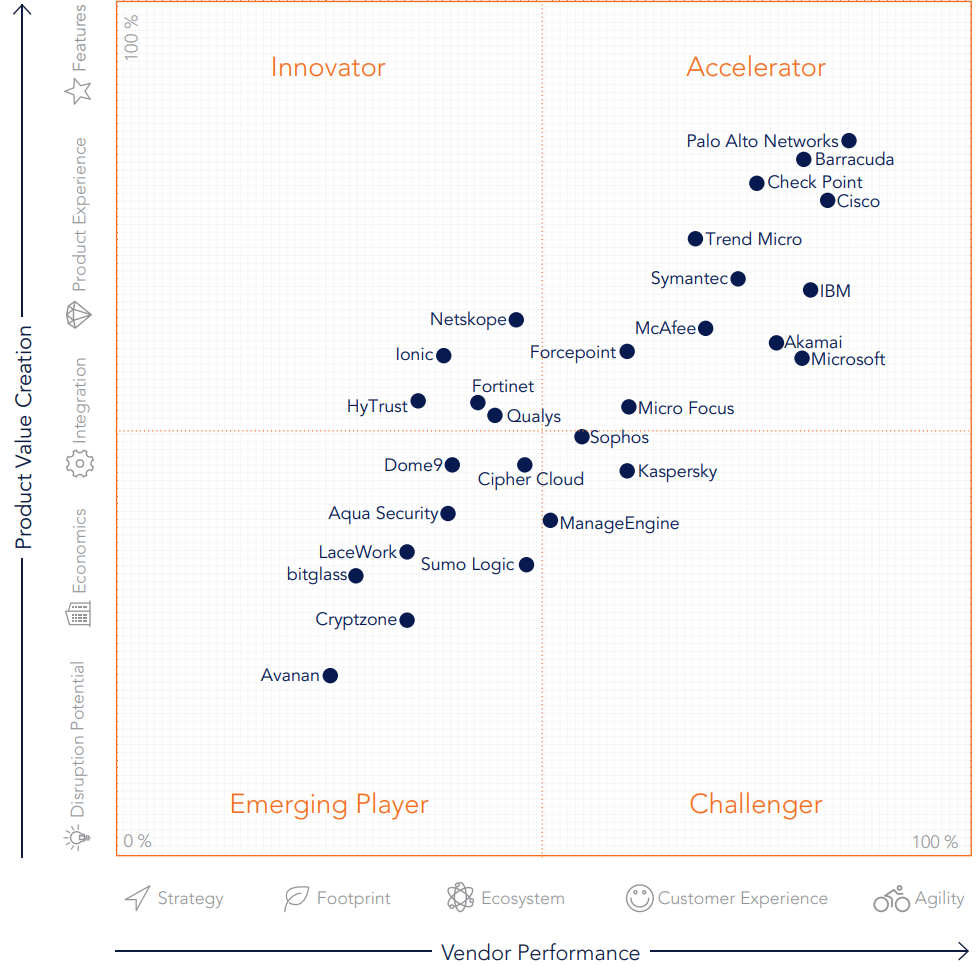
\includegraphics[width=0.8\textwidth]{img/netskopeinnovator.png}
    \caption{Quelle: Crisp Research AG, 2018 - Cloud Security Management Platforms \autocite{Hille2018}}
    \label{fig:netskope}
\end{figure}

\begin{figure}[h]
    \centering
    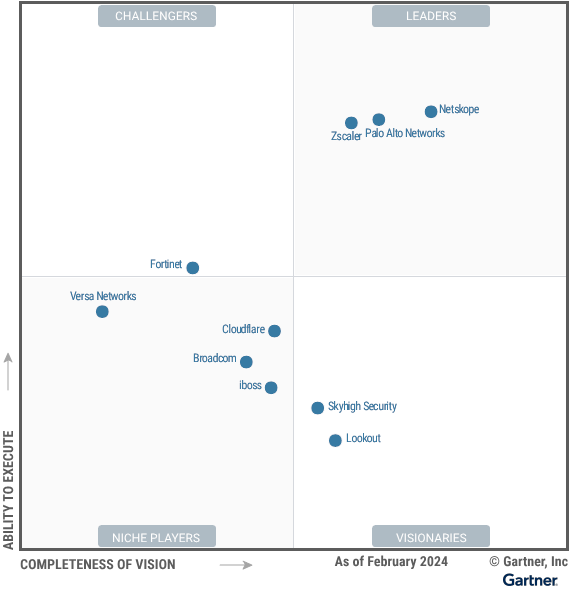
\includegraphics[width=0.8\textwidth]{img/netskope2024.png}
    \caption{Gartner Magic Quadrant voor Security Service Edge (SSE) \autocite{Gartner2024}}
    \label{fig:netskope2024}
\end{figure}


% Netskope onderscheidt zich als een volledig geïntegreerd platform binnen het SASE-framework, met een Secure Service Edge (SSE)-oplossing die DLP, CASB, SWG en ZTNA naadloos combineert. 
% Deze aanpak is waardevol in gedistribueerde werkomgevingen en bij toenemende cloudadoptie \autocite{brouwer2021cloud}. 
% Netskope biedt meer voordelen dan alternatieven zoals Symantec, Digital Guardian, Forcepoint, Microsoft en McAfee. 
% Symantec en Digital Guardian richten zich bijvoorbeeld sterk op endpointbeveiliging, maar missen de cloudfunctionaliteiten die nodig zijn in moderne hybride werkomgevingen. 
% Forcepoint staat bekend om krachtige gedragsanalyses, maar is minder effectief in het ondersteunen van complexe en dynamische cloudomgevingen. 
% Microsoft biedt uitstekende integratie met Office 365, maar hierdoor mist het ook Netskope's cloud-agnostische aanpak, die een breder scala aan cloudapplicaties ondersteunt \autocite{NetskopeTAP2024}. 
% Tenslotte biedt McAfee een breed scala aan beveiligingsoplossingen, maar voor Evolane is Netskope een gebruiksvriendelijker platform met meer flexibiliteit bij het opstellen en aanpassen van regelsets.




% O = onvoldoende
% V = voldoende
% G = goed
% U = uitstekend

% \begin{table}[h]
%     \centering
%     \small
%     \begin{tabular}{p{3cm} p{1.5cm} p{1.5cm} p{1.5cm} p{1.5cm} p{1.5cm} p{1.5cm}}
%         \toprule
%         & \textbf{Cloud-native} & \textbf{SASE/SSE} & \textbf{Flexibele regels} & \textbf{Endpoint focus} & \textbf{SIEM-integratie} & \textbf{Gebruiks\-vriendelijk} \\
%         \midrule
%         Netskope            & U & U & U & U & G & U \\
%         Symantec            & X & X & X & X & G & X \\
%         Microsoft           & X &   &   &   & Vthestral &   \\
%         Forcepoint          & X &   & X & X & G & X \\
%         Digital Guardian    &   &   &   & X &   &   \\
%         McAfee              & X &   & X & X &   &   \\
%         \bottomrule
%     \end{tabular}
%     \caption{Vergelijking van DLP-oplossingen per factor}
%     \label{tab:netskope}
% \end{table}

% Een belangrijke uitdaging bij het implementeren van een Data Loss Prevention (DLP)-oplossing is het omgaan met false positives. 
% Een false positive doet zich voor wanneer een legitieme handeling onterecht als een beveiligingsincident wordt aangeduid. 
% Dit kan leiden tot operationele vertragingen, frustratie bij eindgebruikers en een verlaagde efficiëntie van het systeem. 
% In het geval van Netskope kan een verkeerd geclassificeerd bestand – 
% bijvoorbeeld een legitiem gedeeld rapport dat persoonlijke namen bevat – leiden tot een geblokkeerde workflow of onnodige escalaties.

% Volgens Olateju et al. (2024) vormen false positives een bijzonder knelpunt in AI-gedreven anomaliedetectiesystemen. 
% Hun studie benadrukt hoe een oversensitieve configuratie de nauwkeurigheid verlaagt en tot alertmoeheid leidt bij analisten, 
% wat het risico verhoogt dat echte incidenten over het hoofd worden gezien . 
% Ze stellen tevens dat fine-tuning en continue validatie van modellen essentieel zijn voor het behoud van een werkbare balans tussen veiligheid en gebruiksgemak .

% Ook Lukas (2023) wijst op de uitdagingen van false positives in taalmodellen die worden toegepast in beveiligingscontexten. 
% Zijn onderzoek toont aan dat modellen soms irrelevante of niet-gevoelige informatie als "gevoelig" classificeren, wat leidt tot valse alarmen. 
% Dit is vooral problematisch wanneer DLP-oplossingen gebruik maken van machine learning voor patroonherkenning in natuurlijke taal – 
% iets wat in moderne platforms zoals Netskope steeds vaker het geval is.

% Om deze problematiek te verhelpen, zijn meerdere technieken noodzakelijk:
% Training op domeinspecifieke datasets, zodat modellen context beter begrijpen.
% Gebruik van meerdere detection layers, bijvoorbeeld reguliere expressies in combinatie met ML-gebaseerde detectie.
% Feedback loops, waarin meldingen door gebruikers worden bevestigd of tegengesproken om toekomstige detecties te verbeteren.
% Threshold management, om de gevoeligheid van detectie af te stemmen op bedrijfsbehoeften.
% De balans tussen beveiliging en bruikbaarheid is cruciaal: een te strikte configuratie leidt tot hinder, terwijl een te lakse aanpak risico’s creëert. Netskope biedt hier mogelijkheden tot fijnmazige afstelling, onder andere via confidence levels, policy exceptions en custom DLP rules.
% Kortom, false positives zijn onvermijdelijk in elk geautomatiseerd detectiesysteem, maar door een combinatie van techniek, feedbackmechanismen en zorgvuldig beheer kan hun impact sterk beperkt worden.

% In het onderzoek van Lukas (2023) wordt dieper ingegaan op de problematiek van false positives bij het gebruik van taalmodellen binnen beveiligingscontexten, zoals bij Data Loss Prevention (DLP). Zijn analyse wijst uit dat deze modellen vaak geneigd zijn om ook niet-gevoelige of contextueel irrelevante informatie verkeerd te classificeren als “gevoelig”. Deze overdetectie is problematisch, vooral wanneer modellen op natuurlijke taal getraind zijn en in productieomgevingen zoals Netskope DLP ingezet worden .

% Concreet stelt Lukas dat deze false positives voortkomen uit:
% Overmatige generalisatie van patronen: Het taalmodel associeert bepaalde woordcombinaties (zoals e-mailadressen of namen) automatisch met gevoeligheid, zonder voldoende contextuele verificatie.
% Gebrek aan semantisch onderscheid: De modellen begrijpen onvoldoende het verschil tussen bv. een fictieve naam in een handleiding versus een echte naam in een medisch verslag.
% Bias in trainingsdata: Als de trainingsgegevens oververtegenwoordigd zijn met bepaalde formats of types van informatie, zal het model die patronen als gevoelig beschouwen, ook als dat in de praktijk niet klopt.
% Om deze problematiek te verhelpen, beveelt het onderzoek meerdere technieken aan:
% Context-aware classificatie: In plaats van alleen naar entiteit-types te kijken (zoals "e-mailadres"), moet ook de semantische en syntactische context meewegen.
% Feedback-loops met menselijke evaluatie: Door gebruikers meldingen te laten beoordelen (correct / fout), kan het model bijgestuurd worden.
% Hybride benaderingen: Combinatie van patroon-gebaseerde detectie (regex, heuristieken) en ML om precisie te verhogen.
% Confidence scoring en drempels: Enkel waarschuwingen genereren als het model een hoge mate van zekerheid heeft.

\section{False Positives}
\label{sec:false-positives-literatuurstudie}

False positives bij een DLP-systeem ontstaan wanneer legitieme gegevens onterecht als confidentieel worden geclassificeerd.
Dit kan leiden tot  \textit{\textbf{onnodige waarschuwingen}}, \textit{\textbf{vertragingen in bedrijfsprocessen}} en \textit{\textbf{frustratie bij eindgebruikers}}. 
% Bij overmatige false positives kunnen gebruikers belangrijke waarschuwingen negeren, wat leidt tot \textit{\textbf{alertmoeheid}}.
\textcite{Lukas2023} legt uit dat dit probleem vooral voorkomt in systemen die gebruik maken van machine learning (\gls{ml}) en natuurlijke taalverwerking (\gls{nlp}). 
Dit komt doordat deze systemen vaak niet in staat zijn om de context van gegevens correct te interpreteren, wat leidt tot onjuiste classificaties.
Concreet stelt \textcite{Lukas2023} dat deze false positives vooral voorkomen door:

\begin{itemize}
    \item \textbf{Overmatige generalisatie van patronen}: Het taalmodel associeert bepaalde woordcombinaties, zoals e-mailadressen of namen, automatisch met gevoeligheid, zonder voldoende contextuele verificatie.
    \item \textbf{Gebrek aan semantisch onderscheid}: De modellen begrijpen onvoldoende het verschil tussen bv. een fictieve naam in een handleiding versus een echte naam in een medisch verslag.
   \item \textbf{Bias in trainingsdata}: Als de trainingsgegevens oververtegenwoordigd zijn met bepaalde formats of types van informatie, zal het model die patronen als gevoelig beschouwen, ook als dat in de praktijk niet klopt.
\end{itemize}

\textcite{Olateju2024} stelt vast dat DLP-systemen gemiddeld een false positive-percentage van 4\% tot 5\% vertonen, zelfs bij gebruik van geavanceerde deep learning-algoritmen.
Dit lijkt misschien beperkt, maar in grote organisaties of cloudomgevingen met duizenden datatransacties per dag kan dit resulteren in een aanzienlijke hoeveelheid foutieve waarschuwingen.



% De gevolgen zijn niet louter technisch van aard. 
% False positives leiden tot toegenomen werkdruk voor beveiligingsteams, 
% vertraging van workflows en verminderde gebruikersbetrokkenheid. 
% In het ergste geval ontstaat alertmoeheid, waarbij echte beveiligingsincidenten over het hoofd worden gezien omdat gebruikers of
% analisten gewend raken aan irrelevante meldingen. Dit vergroot het risico op datalekken en non-compliance met wetgeving zoals GDPR of PCI DSS.

% Hoewel volledige eliminatie van false positives onrealistisch is, 
% zijn er diverse manieren om hun impact te beperken. 
% Dit kan via contextuele classificatie, hybride detectiemethoden, 
% en het integreren van gebruikersfeedback in het leerproces van modellen. 
% Moderne platforms zoals Netskope bieden daarnaast concrete instellingen om detectiegevoeligheid te beheren via confidence scores, 
% policy exceptions en maatwerkregels. 
% Door technische, menselijke en beleidsmatige maatregelen te combineren, kan een werkbare balans worden gevonden tussen beveiliging en gebruiksgemak.



% False positives ontstaan wanneer een DLP-systeem onterecht normale gegevens als confidentieel identificeert. 
% Dit kan leiden tot onnodige waarschuwingen en vertragingen in de bedrijfsprocessen.
% Om false positives te vermijden, kan in Netskope bij custom identifiers worden aangegeven dat een bepaald keyword in de buurt moet staan, zoals `RRN' of `Rijksregisternummer'. 
% Hierdoor ziet Netskope het niet als een match of zal het een lagere vertrouwheidsscore geven.
% \autocite{Lukas2023}


% In sectoren zoals de publieke sector en cloud service providers worden grote hoeveelheden gevoelige gegevens verwerkt, w
% aaronder persoonsgegevens (PII) en betalingsgegevens (PCI). 
% Om deze data te beschermen worden Data Leakage Prevention (DLP)-systemen ingezet die gebruikmaken van AI en machine learning om potentieel 
% ongewenste gegevensoverdracht te detecteren. Ondanks technologische vooruitgang kampen deze systemen met een gemiddeld false positive-percentage 
% van circa 4{,}23\%~\cite{detectionaccuracy}. Dit betekent dat een aanzienlijk deel van de gegenereerde waarschuwingen onterecht is, wat verstrekkende
% gevolgen kan hebben voor operationele processen en compliance.

% \subsection{Concreet effect van false positives}
% De aanwezigheid van false positives heeft meerdere negatieve effecten:

% \begin{itemize}
%     \item \textbf{Vertraging van workflows}: Valse meldingen onderbreken bedrijfsprocessen, omdat elke waarschuwing handmatig moet worden gevalideerd. In omgevingen met hoge volumes, zoals overheidsinstanties, leidt dit tot significante vertragingen.
%     \item \textbf{Toegenomen werkdruk}: Security teams worden geconfronteerd met een verhoogde werklast. Onterechte waarschuwingen vergen tijd en middelen die anders besteed zouden worden aan het behandelen van daadwerkelijke incidenten.
%     \item \textbf{Gebruikersfrustratie en verminderde betrouwbaarheid}: Wanneer eindgebruikers regelmatig geconfronteerd worden met valse alarmen, kan dit leiden tot frustratie, verminderde acceptatie van het systeem, en in sommige gevallen zelfs het negeren van belangrijke waarschuwingen (alert fatigue).
%     \item \textbf{Compliance- en veiligheidsrisico's}: Overmatige false positives kunnen ervoor zorgen dat echte datalekken over het hoofd worden gezien. Dit vergroot het risico op non-compliance met regelgeving zoals GDPR of PCI DSS, en kan ernstige gevolgen hebben voor de organisatie.
% \end{itemize}





% Binnen cloudomgevingen en de publieke sector zijn de gevolgen van false positives extra problematisch vanwege de schaal en gevoeligheid van de verwerkte gegevens.
% Hoewel sommige recente studies verbeteringen rapporteren in detectienauwkeurigheid door het gebruik van deep learning 
% (bijv. 3{,}90\% false positives versus 4{,}35\% bij decision trees~\cite{detectionaccuracy}), ligt de focus in de literatuur hoofdzakelijk op technische performance metrics.

% Er is opvallend weinig onderzoek dat zich richt op de operationele impact van deze valse meldingen. 
% Factoren zoals workflowvertraging, menselijke belasting en verminderde gebruikersvertrouwen worden zelden gekwantificeerd, ondanks hun potentiële invloed op de effectiviteit van DLP-systemen.

% \subsection{Onderzoeksnoden en aanbevelingen}

% Deze lacune in de literatuur onderstreept de nood aan meer contextueel onderzoek, met focus op:

% \begin{itemize}
%     \item Het kwantificeren van de operationele impact van false positives in praktijksituaties.
%     \item Het betrekken van eindgebruikers en security professionals in kwalitatieve analyses (zoals casestudies of interviews).
%     \item Het ontwikkelen van verbeterde validatie- en feedbackmechanismen binnen DLP-workflows.
% \end{itemize}
% Toekomstig onderzoek zou de brug moeten slaan tussen technische prestatieverbeteringen en hun reële effect op organisaties. 
% Dit is essentieel om het vertrouwen in DLP-systemen te versterken en de bescherming van PII- en PCI-gegevens in gevoelige sectoren duurzaam te garanderen.




\section{Juridisch kader voor gegevensbescherming in België}%

De bescherming van persoonlijke en bedrijfsinformatie is een essentieel aspect van de hedendaagse digitale samenleving. 
Op zowel nationaal als Europees niveau zijn er wettelijke richtlijnen opgesteld om organisaties te ondersteunen bij het garanderen van de vertrouwelijkheid, 
integriteit en toegankelijkheid van gegevens.

\subsection{Algemene Verordening Gegevens\-besch\-erming (AVG)}%

Dit onderzoek zal in overeenstemming zijn met de Algemene Verordening Gegevensbescherming (AVG of GDPR) 2016/679 van 27 april 2016 \autocite{eu_avg2016} en de Belgische wet van 30 juli 2018 \autocite{BelgischeOverheid2018}.
Volgens de \textcite{eu_avg2016}, overweging (78), moeten passende, technische en organisatorische maatregelen worden genomen om de rechten van natuurlijke personen te beschermen. 
Deze overweging zorgt ervoor dat persoonsgegevens op een veilige en verantwoorde manier worden verwerkt. 
Zo'n beveiliging kan gebeuren door middel van standaardinstellingen die erop zijn gericht om risico's in elke fase van de verwerking van gegevens te minimaliseren.
Op 25 juli 2024 publiceerde de Europese Unie haar tweede verslag over de toepassing van de AVG \autocite{eu_avg2024}. 
Dit rapport legt de nadruk op het feit dat de AVG, ondanks verschillende uitdagingen, een goede basis is voor het veilig en transparant behandelen van persoonsgegevens. 


\subsection{Payment Card Industry Data Security Standard (PCI DSS)}%

De Payment Card Industry Data Security Stand\-ard (PCI DSS) bestaat uit een reeks richtlijnen en regels die ontworpen zijn voor organisaties die betalingsinformatie en kaartinformatie verwerken, 
zoals debit-/ creditcardnummers, Primary Account Numbers (PAN) en Sensitive Authentication Data (SAD), zoals Card Verification Value (CVV) en magnetische stripgegevens, van alle grote kaartsche\-ma's. 
Deze standaard is ontwikkeld om de veiligheid van kaartinformatie te garanderen en vereist dat organisaties maatregelen nemen om de gegevens van kaarthouders te beschermen \autocite{Elluri2018}. 
PCI DSS vereist de implementatie van toegangscontroles, zoals DCS-02 (toegangscontrole tot systemen en gegevens), DCS-07 (beheer van gebruikersidentiteiten en -toegang), 
en DCS-08 (toegangscontrole tot netwerken en systemen), om de veiligheid van kaartinformatie en de bescherming van kaarthoudergegevens te waarborgen \autocite{Elluri2018}.

\subsection{ISO 27001: Informatiebeveiliging}%

Bovendien moet de DLP-oplossing rekening houden met de vereisten van ISO 27001, de internationale norm voor het beheer van informatiebeveiliging. 
In dit verband bespreken \textcite{Alsanabani2020} de noodzaak van DLP-oploss\-ingen die zowel detectie- als preventieve methoden samenbrengen. 
De preventieve aanpak probeert datalekken te vermijden door onder andere het gehele confidentiële bestand te versleutelen, toegangscontrole aan te passen en het labelen van de inhoud.

\subsection{Nationale en Europese richtlijnen}%

Buiten de Belgische wetgeving zijn er ook tal van Europese richtlijnen en nationale standaarden die een belangrijke rol hebben in de bescherming van bedrijfsdata. 
Hierbij kan gedacht worden aan de Algemene Verordening Gegevensbescherming (AVG), de EU Cybersecurity Act en belangrijke Europese richtlijnen, waaronder de NIS2-richtlijn. 
Deze richtlijnen worden verder uitgebreid met specifieke normen, zoals de PCI DSS voor betalingsgegevens en internationale normen, zoals ISO 27001 voor de beveiliging van informatie. 
De NIS2-richtlijn (Richtlijn (EU) 2022/2555), die op 16 januari 2023 is aangenomen door de \textcite{nis2directive}, 
heeft als doel de cyberbeveiliging binnen de EU te versterken door een hoog niveau van beveiliging te waarborgen voor netwerken en informatiesystemen. 
Artikel 21 van de NIS2-richtlijn richt zich op de beveiliging van netwerken en informatiesystemen en legt de verplichting op aan lidstaten om 
ervoor te zorgen dat aanbieders van essentiële en belangrijke diensten passende technische en organisatorische maatregelen nemen. 
Maatregelen die over het DLP-systeem kunnen gaan, zijn onder andere: 

\begin{itemize}
    \item Risicoanalyse (lid 2, punten a en e): Organisaties moeten een risicobeheerproces implementeren dat hen in staat stelt om risico's voor de beveiliging van netwerken en informatiesystemen te identificeren, te evalueren en te beheersen.
    \item Encryptie en toegangscontroles (lid 2, punten h en i): Het gebruik van encryptie, toegangscontroles en regelmatige beveiligingstests en audits.
    \item Incidentenbehandeling (lid 2, punt b): Organisaties moeten procedures en mechanismen hebben voor het detecteren, melden en reageren op beveiligingsincidenten.
    \item Bewustwording en training (lid 2, punt g): Opleidingen om medewerkers te informeren over goede cyberhygiëne en risicomanagement \autocite{nis2directive}. Het DLP-systeem van Netskope staat in voor het trainen van de eindgebruiker, mocht deze iets foutief doen.
\end{itemize}

De studie van \textcite{Nayak2020} geeft een uitgebreid overzicht van systemen voor het detecteren en voorkomen van datalekken, 
inclusief de indeling van systemen op basis van de status van de gegevens (data-at-rest, data-in-motion, dat\-a-in-use) en de detectietechnieken. 
Dit overzicht zal gebruikt worden voor het ontwikkelen van regex-gebaseerde regels in DLP-oploss\-ingen. 
De studie legt de nadruk op het feit dat datalekken zowel onvoorzien als opzettelijk kunnen optreden en geeft uitdagingen aan, 
zoals het identificeren van gevoelige informatie, het balanceren van de detectienauwkeurigheid en de integratie van geavanceerde methodologieën.

% \subsection{Gegevensoverdracht en internationale implicaties}%

\subsection{Andere relevante wetgeving}%

Tabel \ref{tab:wetgeving_dlp} bevat de belangrijkste wettelijke richtlijnen en uitspraken die relevant zijn voor het ontwerp en de implementatie van een Data Leakage Prevention-oplossing voor Belgische bedrijven.

% \begin{figure}
%     \centering
%     % \includegraphics[width=.2\textwidth]
%     \includegraphics[scale=0.50]
%     {img/overzicht.png}
%     \caption{\label{fig:overzicht}Overzicht van de belangrijkste wettelijke richtlijnen en uitspraken voor DLP-oplossingen in België.}
%   \end{figure}

  
  \begin{table}[h]
    \centering
    \small
    \begin{tabular}{p{4cm} p{5cm} p{6cm}}
        \toprule
        \textbf{Wetgeving} & \textbf{Doel} & \textbf{Relevantie voor DLP} \\
        \midrule
        AVG & Bescherming persoonsgegevens & Dataclassificatie en toegangscontrole \\
        PCI DSS & Beveiliging van betalingsgegevens & Encryptie en toegangsbeheer \\
        ISO 27001 & Informatiebeveiliging & Risicoanalyse en ISMS-implementatie \\
        CCB-framework & Strategie voor cybersecurity België & Aanbevelingen voor risicobeheer \\
        NIS2 & Beveiliging netwerken en diensten & Incidentrapportage en risicoanalyse \\
        EU Cybersecurity Act & Certificering van beveiligingstechnologie & DLP-oplossingen certificeren \\
        Schrems II & Gegevensoverdracht naar niet-EU-landen & Beperking van cloud-gebaseerde opslag \\
        \bottomrule
    \end{tabular}
    \caption{Overzicht van wetgeving en relevantie voor DLP}
    \label{tab:wetgeving_dlp}
\end{table}


  

\section{Ethische overwegingen}%

Een essentieel aspect van de implementatie van DLP is het vinden van de juiste balans tussen gegevensbeveiliging en gebruikersprivacy. 
Het gebruik van DLP-systemen kan leiden tot het monitoren van gebruikersgedrag, wat kan worden gezien als een inbreuk op de privacy van medewerkers. 
Om het vertrouwen bij medewerkers en klanten te behouden, is het belangrijk om transparant te zijn over het gebruik van DLP-systemen en de redenen daarvoor. 
Hierdoor weet elke gebruiker welke gegevens worden verzameld en hoe deze worden gebruikt \autocite{Zaini2024}. 
Deze regelsets moeten niet alleen voldoen aan de wettelijke vereisten, maar ook aan de ethische normen en waarden van de organisatie. 
Om monitoring van data en gebruikersgedrag te minimaliseren, 
zal de implementatie van de DLP-oplossing specifiek gericht zijn op het beschermen van gevoelige gegevens en het voorkomen van datalekken. 

Tijdens het vak \textit{IT Professional \& Career Orientation (ITPCO)} kwam het belang van ethische en juridische aspecten binnen informatieveiligheid uitgebreid aan bod. 
Gastspreker \textcite{SoficoGuestLecture2024} van \textit{Sofico} presenteerde een overzicht van hoe een internationaal bedrijf dat softwareoplossingen ontwikkelt voor autofinanciering, 
leasing, fleetmanagement en mobiliteitsbeheer, privacy en compliance structureel integreert in zijn processen \autocite{SoficoGuestLecture2024}. 
Het gastcollege behandelde onder meer fysieke beveiligingsmaatregelen, toegangsbeheer tot ontwikkelomgevingen en de inzet van white hat hackers voor het identificeren van kwetsbaarheden.
De organisatie gebruikt principes zoals \textit{Privacy by Design} en \textit{Security by Design} binnen de volledige ontwikkeling en implementatie van software. 
Deze principes staan in lijn met de \gls{avg} en \gls{iso} normen, waarbij de focus ligt op het minimaliseren van gegevensverwerking en het behouden van de privacy van gebruikers.
De inzichten van Sofico zijn rechtstreeks van toepassing op dit onderzoek.
\textit{Privacy by Design} en \textit{Security by Design} zijn namelijk gericht op minimale gegevensverwerking, transparantie, logging en traceerbaarheid. 
Binnen \textcite{Netskope2024PrivByDesign} worden deze principes toegepast via \textit{\textbf{in-memory verwerking}}, \textit{\textbf{gegevensobfuscatie}}, \textit{\textbf{klantgecontroleerde datalokalisatie}} en \textit{\textbf{uitgebreide transactie-logging}}.

% Tijdens het vak \textit{IT Professional \& Career Orientation (ITPCO)} werd aandacht besteed aan de ethische, 
% juridische en organisatorische aspecten van gegevensverwerking en informatieveiligheid. 
% Deze inzichten zijn rechtstreeks van toepassing op dit onderzoek, 
% dat zich toespitst op de implementatie van een DLP-oplossing binnen een cloud- en compliancegevoelige omgeving.

% Een bijzonder waardevol onderdeel van het vak was het gastcollege door een medewerker van Sofico, 
% een internationaal softwarebedrijf actief binnen de automotive-sector. 
% Dit college illustreerde hoe bedrijven zoals Sofico concreet omgaan met databeveiliging, 
% toegangsbeheer en regelgeving zoals de AVG en ISO/IEC 27001. De spreker benadrukte onder andere het belang van:

% \begin{itemize}
%   \item \textbf{Data Classification en Secure Development:} het correct classificeren en beveiligen van data over de volledige softwareontwikkelingscyclus, conform het principe van \textit{Privacy by Design}.
%   \item \textbf{Datalekken en verantwoordelijkheden:} een datalek moet binnen 24 uur gemeld worden aan de bevoegde autoriteiten (zoals de GBA in België). Hiervoor zijn rollen zoals de \textit{Data Protection Officer (DPO)} essentieel.
%   \item \textbf{\gls{iso}-certificatie:} organisaties worden via deze norm verplicht om informatieveiligheid systematisch aan te pakken. Topics zoals thuiswerken, wachtwoordbeheer, netwerkstructuren en leveranciersbeheer worden hierbij geëvalueerd.
% \end{itemize}

% Deze inzichten waren bijzonder relevant gezien mijn bachelorproef een DLP-oplossing onderzoekt die PII/PCI-gegevens in de cloud moet beschermen. 
% Vanuit ethisch oogpunt is het cruciaal om dataminimalisatie, transparantie en toestemming (\textit{lawfulness, fairness, transparency}) 
% centraal te plaatsen in zowel ontwerp als configuratie. 
% Daarnaast vormde het college een reflectiemoment: in welke mate houdt mijn stagebedrijf zelf rekening met deze normen en 
% is het bewust van certificeringsvereisten zoals ISO/IEC 27001?
